\documentclass{thesisclass}
% Based on thesisclass.cls of Timo Rohrberg, 2009
% ----------------------------------------------------------------
% Thesis - Main document
% ----------------------------------------------------------------


%% -------------------------------
%% |  Information for PDF file   |
%% -------------------------------
\hypersetup{
 pdfauthor={Not set},
 pdftitle={Not set},
 pdfsubject={Not set},
 pdfkeywords={Not set}
}


%% ---------------------------------
%% | Information about the thesis  |
%% ---------------------------------

\newcommand{\myname}{Name}
\newcommand{\mytitle}{Title of thesis\\ 
											Second title line}
\newcommand{\myinstitute}{Institute for Program Structures\\
													and Data Organization (IPD)}

\newcommand{\reviewerone}{?}
\newcommand{\reviewertwo}{?}
\newcommand{\advisor}{?}
\newcommand{\advisortwo}{?}

\newcommand{\timestart}{XX. Monat 20XX}
\newcommand{\timeend}{XX. Monat 20XX}
\newcommand{\submissiontime}{DD. MM. 20XX}


%% ---------------------------------
%% | ToDo Marker - only for draft! |
%% ---------------------------------
% Remove this section for final version!
\setlength{\marginparwidth}{20mm}

\newcommand{\margtodo}
{\marginpar{\textbf{\textcolor{red}{ToDo}}}{}}

\newcommand{\todo}[1]
{{\textbf{\textcolor{red}{(\margtodo{}#1)}}}{}}


%% --------------------------------
%% | Old Marker - only for draft! |
%% --------------------------------
% Remove this section for final version!
\newenvironment{deprecated}
{\begin{color}{gray}}
{\end{color}}


%% --------------------------------
%% | Settings for word separation |
%% --------------------------------
% Help for separation:
% In german package the following hints are additionally available:
% "- = Additional separation
% "| = Suppress ligation and possible separation (e.g. Schaf"|fell)
% "~ = Hyphenation without separation (e.g. bergauf und "~ab)
% "= = Hyphenation with separation before and after
% "" = Separation without a hyphenation (e.g. und/""oder)

% Describe separation hints here:
\hyphenation{
% Pro-to-koll-in-stan-zen
% Ma-na-ge-ment  Netz-werk-ele-men-ten
% Netz-werk Netz-werk-re-ser-vie-rung
% Netz-werk-adap-ter Fein-ju-stier-ung
% Da-ten-strom-spe-zi-fi-ka-tion Pa-ket-rumpf
% Kon-troll-in-stanz
}


%% ------------------------
%% |    Including files   |
%% ------------------------
% Only files listed here will be included!
% Userful command for partially translating the document (for bug-fixing e.g.)
\includeonly{%
titlepage,
declaration,
introduction,
content,
evaluation,
conclusion,
appendix
}


%%%%%%%%%%%%%%%%%%%%%%%%%%%%%%%%%
%% Here, main documents begins %%
%%%%%%%%%%%%%%%%%%%%%%%%%%%%%%%%%
\begin{document}

% Remove the following line for German text
\selectlanguage{english}

\frontmatter
\pagenumbering{roman}
%% titlepage.tex
%%

% coordinates for the bg shape on the titlepage
\newcommand{\diameter}{20}
\newcommand{\xone}{-15}
\newcommand{\xtwo}{160}
\newcommand{\yone}{15}
\newcommand{\ytwo}{-253}

\begin{titlepage}
% bg shape
\begin{tikzpicture}[overlay]
\draw[color=gray]  
 		 (\xone mm, \yone mm)
  -- (\xtwo mm, \yone mm)
 arc (90:0:\diameter pt) 
  -- (\xtwo mm + \diameter pt , \ytwo mm) 
	-- (\xone mm + \diameter pt , \ytwo mm)
 arc (270:180:\diameter pt)
	-- (\xone mm, \yone mm);
\end{tikzpicture}
	\begin{textblock}{10}[0,0](4,2.5)
		
\includegraphics[width=.3\textwidth]{logos/KITLogo_RGB.pdf}
	\end{textblock}
	\changefont{phv}{m}{n}	% helvetica	
	\vspace*{3.5cm}
	\begin{center}
		\Huge{\mytitle}
		\vspace*{2cm}\\
		\Large{
			\iflanguage{english}{Diploma Thesis of}			
												  {Diplomarbeit\\von}
		}\\
		\vspace*{1cm}
		\huge{\myname}\\
		\vspace*{1cm}
		\Large{
			\iflanguage{english}{At the Department of Physics}			
													{An der Fakult\"at f\"ur Informatik}
			\\
			\myinstitute
		}
	\end{center}
	\vspace*{1cm}
\Large{
\begin{center}
\begin{tabular}[ht]{l c l}
  % Gutachter sind die Professoren, die die Arbeit bewerten. 
  \iflanguage{english}{Reviewer}{Erstgutachter}: & \hfill  & \reviewerone\\
  \iflanguage{english}{Second reviewer}{Zweitgutachter}: & \hfill  & \reviewertwo\\
  \iflanguage{english}{Advisor}{Betreuender Mitarbeiter}: & \hfill  & \advisor\\
  \iflanguage{english}{Second advisor}{Zweiter betreuender Mitarbeiter}: & \hfill  & \advisortwo\\
  % Der zweite betreuende Mitarbeiter kann weggelassen werden. 
\end{tabular}
\end{center}
}


\vspace{2cm}
\begin{center}
\large{\iflanguage{english}{Duration:}{Bearbeitungszeit}: \timestart \hspace*{0.25cm} -- \hspace*{0.25cm} \timeend}
\end{center}


\begin{textblock}{10}[0,0](4,16.8)
\tiny{ 
	\iflanguage{english}
		{KIT -- University of the State of Baden-Wuerttemberg and National Research Center of the Helmholtz Association}
		{KIT -- Universit\"at des Landes Baden-W\"urttemberg und nationales Forschungszentrum in der Helmholtz-Gemeinschaft}
}
\end{textblock}

\begin{textblock}{10}[0,0](14,16.75)
\large{
	\textbf{www.kit.edu} 
}
\end{textblock}

\end{titlepage}

\vspace*{36\baselineskip}
\hbox to \textwidth{\hrulefill}
\par
Ich versichere wahrheitsgem\"a\ss, die Arbeit selbstst\"andig angefertigt, alle benutzten Hilfsmittel vollst\"andig und genau angegeben und alles kenntlich gemacht zu haben, was aus Arbeiten anderer unver\"andert oder mit Ab\"anderungen entnommen wurde.

\textbf{PLACE, DATE}
\vspace{1.5cm}

\dotfill\hspace*{8.0cm}\\
\hspace*{2cm}(\textbf{YOUR NAME}) %center name with hspace

\thispagestyle{empty}
\blankpage


%% -------------------
%% |   Directories   |
%% -------------------
\tableofcontents
\blankpage


%% -----------------
%% |   Main part   |
%% -----------------
\mainmatter
\pagenumbering{arabic}
%% introduction.tex
%%

%% ==============================
\chapter{Introduction}
\label{ch:Introduction}
%% ==============================
    \section{Neutrinos in the standard model}
    \label{ch:Introduction:sec:Neutrinos in the standard model}
    During the second part of the 20th century, a model stating 16 particles has been developed to describe a huge portion of known phenomena, the standard model. It contains six quarks, six leptons (both made up of three particle generations) and four types of Gauge Bosons. The latter are carriers of the standard models interactions of the former particles, meaning all interactions of matter are based on the exchange of one or more of the Gauge Bosons. 
    For our universe, gravity, the graviton generated force, plays a major role for formation and stability af almost all larger structures. In particle physics however, it can mostly be neglected. Here, only the strong and weak as well as the electromagnetic interaction make for noticable contributions to phenomena observed. That is why, in the standard model, gravity as well as its carrier, the graviton, are neglected.
    Most of what we can observe with our bare eyes or in basic experiments is attributable to the electromagnetic force or gravity, however, strong and weak interaction do play a major role when it comes to high energy physics. Here, the limited reach of the two is overcome by small distances between interacting particles. In case of the neutrino, detection and by that the study of its characteristics is even more difficult as it interacts only gravitationally and weakly. Now, as mentioned before, gravity is indeed long range, but very weak in force. And although weak intraction is a lot stronger compared to gravity, it is still weak compared to both electromagnetic and strong interactions. That is why the neutrino is considered elusive, detection efficiencies are low and only large scale detectors are able to detect statistically relevant amounts of neutrinos.
    One method used quite frequently is the Cherenkov radiation emitted while travelling through matter at speeds above the speed of light. This light, comparable to the supersonic cones planes cause in air, can be detected by standard photomiltiplier tubes. The problem is that, as mentioned above, the volumes to be able to make dependable statements on directions and energies need to be large. This is why most experiments make use of ``natural'' detectors such as water \todo{cite MARE+ICE Cube} or even ice.
    Other approaches are to catch neutrinos in reactions where those are required such as inverse beta decays:
    \begin{equation}
		\ce{\bar\nu_e + p -> e^+ + n}
    \end{equation}
   
    
    In the standard model, neutrinos are considered massless. 
    Many experiments though have shown that the weightless neutrino is a wrong assumption. Most of these were experiments prooving neutrino oscillatinos with both reactor neutrinos and solar neutrinos such as Kamiokande\cite{PhysRevLett.110.181802} or SNO \cite{SNOOscillations} \todo{add experiments}.
    Important for those experiments is the known source location making baseline analysis possible.
    
    Up till now, only the differences of the squared masses are known. This leads to different relations depending on how masses are distributed between the flavours, \ref{fig:massSchemes}, and how large they are absolutely \ref{fig:massHierarchy}. This problem is solved by the knowledge of one of the masses. KATRIN is on the verge of finding the $\nu_e$'s mass.\cite{becker2008a}
    
    \begin{figure}
    \centering
    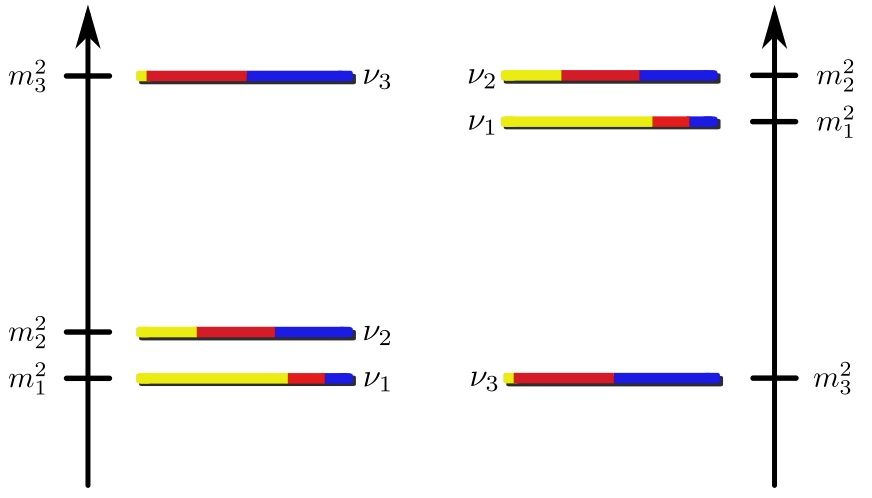
\includegraphics[width=0.5\textwidth]{graphics/standardModel/massHierarchy.jpg}
    	 \caption[Neutrino mass hierarchy]{The possible mass hierarchies for neutrinos.}
    	\label{fig:massSchemes}
    \end{figure}
    \begin{figure}
	\caption[Neutrino mass areas]{Possible mass areas}
    	\label{fig:massHierarchy}
    \end{figure}

    
    \subsection{Neutrino Oscillations}
    \label{ch:Introduction:sec:Massive neutrino:subsec:neutrino Oscillations}
      If the neutrinos were without mass, its mass eigenstates would equal its flavour eigenstates:
      
    \begin{equation}
	\begin{array}{ccc}
      	|\nu_e>		& = & |\nu_1>\\
      	|\nu_\mu>	& = & |\nu_2>\\
      	|\nu_\tau>	& = & |\nu_3>\\
    	 \end{array}
    \end{equation}
    First doubts concerning this asumptions occured as inconsistencies between the measured and the calculated solar $\nu$-flux occured. As the count on $\nu_e$ was too low, the theory of neutrino oscillations emerged, stating that a mixture of flavours was possible as the flavours were made up of all three of the mass eigenstates. The mixture is described by the so called Pontecorvo-Maki-Nakagawa-Sakata matrix:
        \begin{equation}
        \left(
        \begin{array}{c}
	  |\nu_e>\\
	  |\nu_\mu>\\
	  |\nu_\tau>\\
        \end{array}
        \right)
	 = \left(
	\begin{array}{ccc}
      	\theta_{e,1} & \theta_{e,2} & \theta_{e,3}\\
      	\theta_{\mu,1} & \theta_{\mu,2} & \theta_{\mu,3}\\
      	\theta_{\tau,1} & \theta_{\tau,2} & \theta_{\tau,3}\\
      	\end{array}
	\right)
	\left(
	\begin{array}{c}
      	|\nu_1>\\
      	|\nu_2>\\
      	|\nu_3>\\
    	 \end{array}
    	 \right)
    \end{equation}
    
    \subsection{Direct measurement of neutrino mass}
    \label{ch:Introduction:sec:Massive neutrino:subsec:direct Neutrino Mass measurement}
    Direct measurements of the neutrino mass require a reaction known to include neutrinos in its equation. There are both spectrometric and calorimetric approaches. While the scale of spectrometers is getting bigger and bigger, calorimetric approaches seem to be a reasonable alternative, although the slow detector response - the detector material itself is decaying - requires for large arrays of detectors leading to extensive space requirements as well at some point. The luminosity of spectrometer experiments though is unachieved by any other. That is why the KATRIN collaboration is working on a setup to measure electrons from Tritium decay to determine the neutrino mass. 
     
    \subsection{Indirect measurement of neutrino mass}
    \label{ch:Introduction:sec:Massive neutrino:subsec:indirect Neutrino Mass measurement}
    Another approach is using indirect ways of finding the neutrino mass. One possibility here is to search for neutrinoless double beta decay, $0\nu\beta\beta$, which can exist only if the neutrino is its own anti-particle, a so called majorana neutrino. Then, if two nuclei beta decay, the neutrino from one vertex can be absorbed in the second as an anti-neutrino - or vice versa. The decay would then not emit any neutrino and the rate would be dependant on the effective Majorana neutrino mass square'' \cite{currentNeutrinoSearches}:
    \begin{equation}
    	\Gamma_{0\nu\beta\beta} \propto \left| \sum{U_{ei}^2m\left(\nu_i\right)}\right|^2
    \end{equation}

    
    \section{Cosmic muons and their interaction with matter}
    \label{ch:introduction:sec:Cosmic Air Showers}
    When high energy particles hit the upper parts of the atmosphere, a cascade of particles generated from the interaction with atmospheric molecules and atoms follows. Most primary particles are nucleons, most of which again are free protons, i.e. Hydrogen ions. Helium nucleons' fluxes are already about a order of magnitude below that, higher mass number nuclei show even lower rates\cite{highEnergyCosmicRays}. 
    \begin{figure}
	\begin{minipage}[d]{0.49 \textwidth}
		  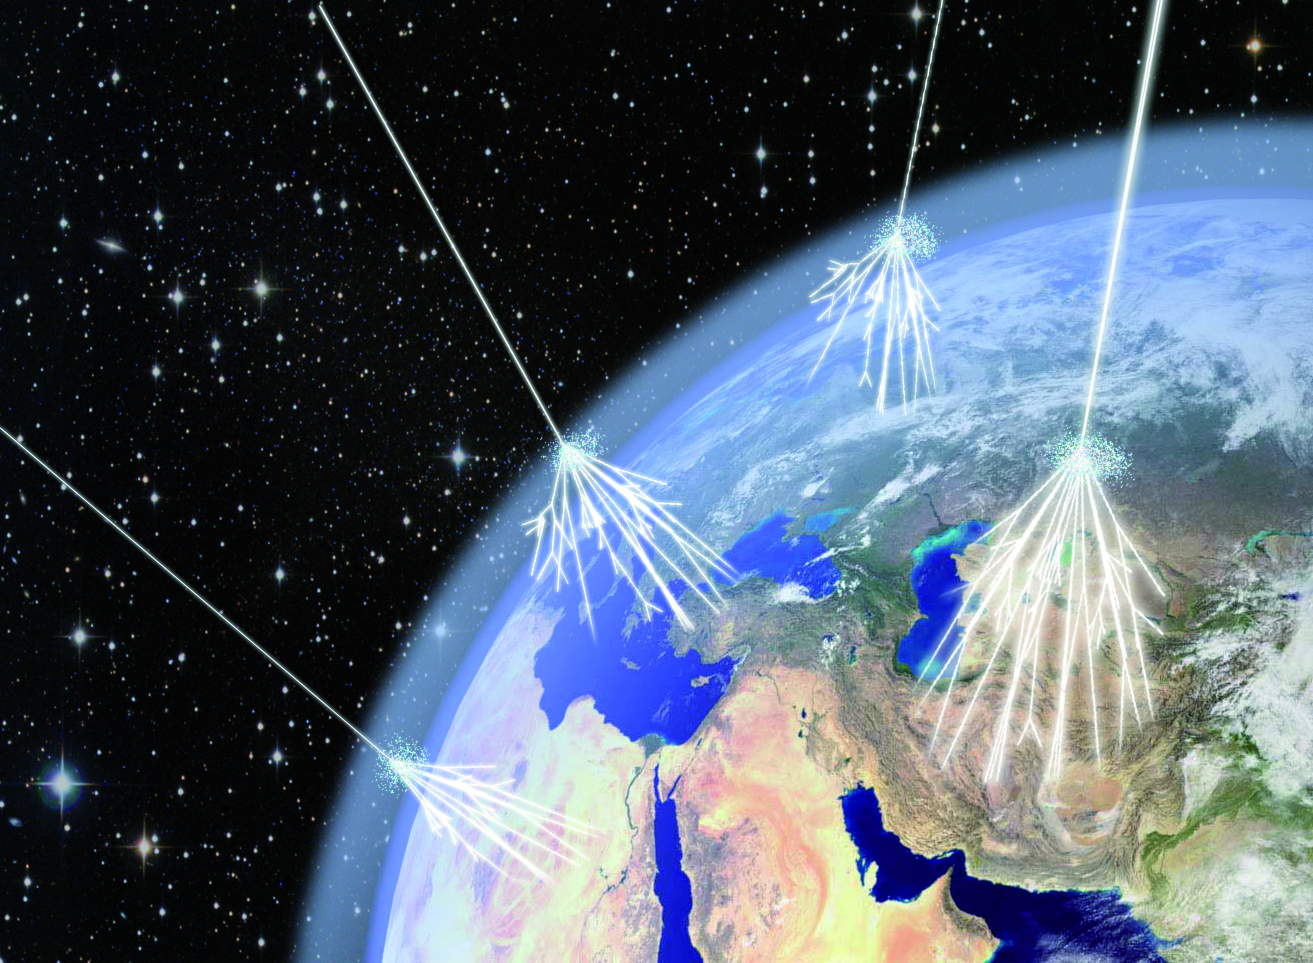
\includegraphics[width=\textwidth]{graphics/cosmicRays/cosmicRays.jpg}
	\end{minipage}
	\begin{minipage}[d]{0.49 \textwidth}
		  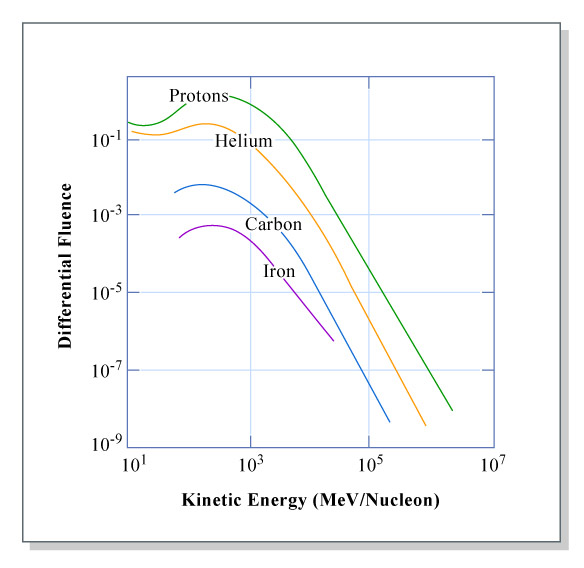
\includegraphics[width=\textwidth]{graphics/cosmicRays/energySpectrum.jpg}
	\end{minipage}
	\caption[Cosmic ray composition]{On the left, an artistic impression of various cosmic rays hitting the atmosphere \cite{airShower}. On the right, the measured composition for cosmic nuclei is shown: on top, the lightest particle, the proton. further down, all with orders of magnitude smaller rates, heavier ions.}
    \end{figure}
    \todo{insert right side graphic from TODOR}
    By different interactions, secondary partcles are created. Any particle satisfying the inequation \begin{equation}
      E_{sec,kin} + m_{sec} c^2 < E_{prim,kin} + m_{prim}
    \end{equation}
    can be created. Mostly pions at first, those cascade further. Often through intermediate photons, muons emerge. These travel towards the earths surface mostly close to the speed of light due to their small masses though high energies. Even at these high speeds, the muons' average decay time of around \SI{2.2}{\micro\second} \cite{muonLifetime} is too small for many muons to reach the earth's surface from our reference frame's point of view. In the most common production height of \SI{2}{\kilo\meter} \cite{muonProductionHeight}, the non relativistic time of flight for a \SI{90}{\percent} speed of light particle would be
    \begin{equation}
	t_{class} = \SI{2}{\kilo\meter} / 0.9\cdot c = 
    \end{equation}
    meaning only time dilation from special relativity makes the muon flux as large as ist is:
    \begin{equation}
    	t_{rel} = t_{class} / \sqrt{1-0.9^2}
    \end{equation}
    which, from our reference frame, prolongs the lifetime by a factor of around 5, being already enough to reach the surface from heights of \SI{3}{\kilo\meter}. Most muons have even higher energies, making it possible for them to reach surface from greater heigts and under non perpendicular angles towards it.
    For KATRIN, this poses a problem. A smaller flux would be advantageous, as muons may, through different kinds of interaction, cause emission of electrons from the spectrometer vessels surface. Shielding against muons is difficult as it requires thick layers of dense matter due to the muons high energies and the low deposition in matter in relations to those. 
    


%% content.tex
%%

%% ==============
\chapter{Content Chapter 1}
\label{ch:Content1}
%% ==============

The content chapters of your thesis should of course be renamed. How many chapters you need to write depends on your thesis and cannot be said in general. 

Check our the examples theses in the Wiki. 

Of course, you can split this .tex file into several files if you prefer. 


%% ===========================
\section{Section 1}
\label{ch:Content1:sec:Section1}
%% ===========================

\dots


%% ===========================
\section{Section 2}
\label{ch:Content1:sec:Section2}
%% ===========================

\dots


%% content.tex
%%

%% ==============
\chapter{Content Chapter 2}
\label{ch:Content1}
%% ==============

\dots


%% ===========================
\section{Section 1}
\label{ch:Content2:sec:Section1}
%% ===========================

\dots


%% ===========================
\section{Section 2}
\label{ch:Content2:sec:Section2}
%% ===========================

\dots

Add additional content chapters if required. 
%% evaluation.tex
%%

%% ==================
\chapter{Evaluation}
\label{ch:Evaluation}
%% ==================

\dots


%% ===============================
\section{Section 1}
\label{ch:Evaluation:sec:Section1}
%% ===============================

\dots


%% ===============================
\section{Section 2}
\label{ch:Evaluation:sec:Section2}
%% ===============================

\dots


%% ===============================
\section{Section 3}
\label{ch:Evaluation:sec:Section3}
%% ===============================

\dots
%% conclusion.tex
%%

%% ==================
\chapter{Conclusion \& Outlook}
\label{ch:Conclusion}
KATRIN is moving forward to finding the neutrino mass - and another part contributing to the whole experiment has been completed with the muon detection system operational and taking data. 
At the main spectrometer, set up has been completed. The monitor spectrometer system was readopted. Both systems are able to take data at rates that compare well to literature values and simulations.
Many settings had to be adjusted for the detection system to realize its full potential. High voltage supplies were installed, software settings within the ORCA software were adapted to the system's needs and synchronization with the FPD was set up.
In the commissioning phase for the muon detection system, different tests were performed to ensure a smoothly working system. The single PMTs were tested with a Sr source revealing two sides showing lower rates than the rest. This was compensated for by raising acceleration voltages for the affected sides. The stability of the system was investigated. It was found that natural atmospheric fluctuations cause much larger rate fluctuations than the module electronics. The efficiency of the single modules was examined and found to be \SI{93.4 \pm 3.4}{\percent}. The module's rates compare very well to literature values. 

It was shown that the muon induced electron rate is well shielded by axially symmetric magnetic fields and that, under different conditions, this rate increases strongly. This proved that the great efforts invested to achieve accurate field knowledge and settings are necessary and will be rewarded with low background measurements.
Analysis with both asymmetric and non axially symmetric fields were very successful showing that all induced events show similar times of flight from the vessel wall to the detector. At the main spectrometer, the setup still needs to be optimized. Due to the limited measurement time in the now ended SDS commissioning measurement phase, further Investigation of the Problem was not possible but will be in the future.






%% --------------------
%% |   Bibliography   |
%% --------------------
\cleardoublepage
\phantomsection
\addcontentsline{toc}{chapter}{\bibname}

\iflanguage{english}
{\bibliographystyle{IEEEtranSA}}	% english style
{\bibliographystyle{babalpha-fl}}	% german style
												  
% Use IEEEtran for numeric references
%\bibliographystyle{IEEEtranSA})

\bibliography{thesis}


%% ----------------
%% |   Appendix   |
%% ----------------
\cleardoublepage

%% appendix.tex
%%

%% ==============================
%\chapter{Appendix}
%\label{ch:Appendix}
%% ==============================

\appendix

\iflanguage{english}
{\addchap{Appendix}}	% english style
{\addchap{Anhang}}	% german style


\section{First Appendix Section}
		\label{Anhang-Implementierung}
		
\setcounter{figure}{0}
		
\begin{figure} [ht]
  \centering
   ein Bild
  \caption{A figure}
  \label{fig:BPMNBeispiela}
\end{figure}


\begin{figure} [ht]
  \centering
    %\includegraphics{graphics/ORCA/script}
  \caption{Scripting task through the example of a LFCS current ramping script. All currents are incremented in thenths of the maximum current for the individual coil. }
  \label{fig:ORCA:script}
\end{figure}

\dots






\end{document}
